\textbf{Cas d'utilisation: Payer avec une carte d'abonnement}

\textbf{Acteur primaire:} Le conducteur

%\textbf{Acteur support:}

\textbf{Pré-condition: }  la borne affiche le montant

 
%\textbf{Post-condition: } 

\textbf{Scenario primaire: } \\
    \textbf{1.} Le conducteur insère sa carte d’abonnement pour payer. \\
    \textbf{2.} La borne enregistre le passage sur l’ordinateur centrale.\\
    \textbf{3.} Le conducteur récupère sa carte.\\

\textbf{Variantes:}\\
    \textbf{1a.}Le conducteur insère une carte invalide, un technicien est appelé.\\
    
%\textbf{Décomposition des cas d'utilisation:} 
%\begin{figure}[h]
 %   \centering
  %  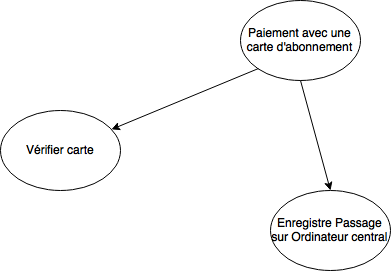
\includegraphics[scale=0.7]{02_Desenvolvimento/TD2/images/PaiementCarteAbonnement.png}
   % \caption{Décomposition des cas d'utilisation: Payer avec une carte d'abonnement}
%\end{figure}
